\documentclass[11pt, a4paper, leqno]{article}
\usepackage{a4wide}
\usepackage[T1]{fontenc}
\usepackage[utf8]{inputenc}
\usepackage{float, afterpage, rotating, graphicx}
\usepackage{epstopdf}
\usepackage{longtable, booktabs, tabularx}
\usepackage{fancyvrb, moreverb, relsize}
\usepackage{eurosym, calc}
% \usepackage{chngcntr}
\usepackage{amsmath, amssymb, amsfonts, amsthm, bm}
\usepackage{caption}
\usepackage{mdwlist}
\usepackage{xfrac}
\usepackage{setspace}
\usepackage[dvipsnames]{xcolor}
\usepackage{subcaption}
\usepackage{minibox}
% \usepackage{pdf14} % Enable for Manuscriptcentral -- can't handle pdf 1.5
% \usepackage{endfloat} % Enable to move tables / figures to the end. Useful for some
% submissions.

\usepackage[
    natbib=true,
    bibencoding=inputenc,
    bibstyle=authoryear-ibid,
    citestyle=authoryear-comp,
    maxcitenames=3,
    maxbibnames=10,
    useprefix=false,
    sortcites=true,
    backend=biber
]{biblatex}
\AtBeginDocument{\toggletrue{blx@useprefix}}
\AtBeginBibliography{\togglefalse{blx@useprefix}}
\setlength{\bibitemsep}{1.5ex}
\addbibresource{refs.bib}

\usepackage[unicode=true]{hyperref}
\hypersetup{
    colorlinks=true,
    linkcolor=black,
    anchorcolor=black,
    citecolor=NavyBlue,
    filecolor=black,
    menucolor=black,
    runcolor=black,
    urlcolor=NavyBlue
}


\widowpenalty=10000
\clubpenalty=10000

\setlength{\parskip}{1ex}
\setlength{\parindent}{0ex}
\setstretch{1.5}


\begin{document}

\title{Convolutional Neural Networks and Satellite Imagery for Economic Analysis \thanks{M.Danial Syed, Bonn University. Email: \href{mailto:s6musyed@uni-bonn.de}{\nolinkurl{s6musyed [at] uni-bonn [dot] de}}.}}

\author{M.Danial Syed}

\date{
    \today
}

\maketitle


\begin{abstract}
\noindent This term paper shows how deep learning can be used alongside satellite imagery and traditional survey data to quantify economic outcomes. The specific example I follow is from the study \textit{Combining satellite imagery and machine learning to predict poverty} by \citet{jean2016combining} to predict poverty in Malawi using consumption expenditure. The key contribution of this replication project is to conduct data management, model training, and prediction in a reproducible and accessible way since the original study and related works required considerable manual effort to reproduce results. In doing so, this project draws on concepts from this course, particularly in relation to managing large projects, and demonstrates Python's rich scientific libraries in the process, thus providing a suitable platform for users to easily scale up this work.
\end{abstract}

\clearpage


\section{Introduction} % (fold)
\label{sec:introduction}
test
A key challenge in tracking progress on poverty eradication goals is the unusual difficulty of obtaining administrative survey data in many regions most affected by poverty. This unavailability is due to the time-consuming and cost-prohibitive nature of conducting large-scale surveys. At the same time, any serious progress on poverty eradication goals necessitates that we are able track poverty in a timely and reliable manner. This calls for innovative modeling techniques to bridge this data gap by drawing on cheap and abundant sources of data as an alternative to household surveys, to track economic outcomes.

The current replication project examines one way to do this following \citet{jean2016combining} by using deep learning along with high resolution daytime satellite imagery and nightlight data to quantify poverty in Malawi. Since satellite imagery does not explicitly capture the vast differences in wealth between regions of a country, transfer learning is deployed to help the model extract economically relevant features from thousands of unstructured satellite images. More specifically, higher nightlights intensity typically indicates a given region is more developed than a region with lower nightlights. This nightlight data can be used to extract landscape features in daytime imagery that are correlated with economic outcomes, such as roads, farmlands, waterways, roof, and urban areas. In the final step, the trained model can be used to predict village level wealth as measured by traditional surveys. 

The contribution of this project is to create a seamless, reproducible workflow for  \textit{Combining satellite imagery and machine learning to predict poverty} \citep{jean2016combining} to show how satellite imagery can be easily integrated into economists' research and programming pipelines. Currently, the layout of the original replication kit and related repositories on Github involve considerable work to obtain and manage the data, and run several scripts in a particular order to produces the desired results. This complexity may disincentivize the ability of new users to alter model parameters and build on the work. I ameliorate this issue by integrating all scripts and tasks in a coordinated `pytask` framework. In doing so, I utilize the CNN method to estimate consumption expenditure in Malawi and attempt to match the $R^2$ from the authors' model, with an emphasis on highlighting the several programming steps involved in such an analysis, from data collection to prediction. 

\subsection{Convolutional Neural Networks (CNN)}

The deep learning method used is CNN, which is a class of artificial neural network (ANN) in deep learning. However, what makes CNN so unique relative to other types of networks is their superior performance in analyzing visual imagery since CNN architectures operate under the implicit assumption that the inputs are image-like. This makes them well-suited to image classification and object recognition tasks such as ours.

\textbf{Convolutional Layer} - These layers are the foundation of any CNN. Suppose we provide an input in the form of a satellite image - since this image is made up of pixels, it will consist of a matrix of pixels that indicate the RGB of the image. The input will thus hold the raw pixel values of the image (for example, an image of width 32, height 32, and three color channels R,G,B). Then, a filter consisting of learnable parameters acts as a feature detector and scans over the input volume and checks if a feature is present. Every filter has a small size, but covers the entire depth of the input volume. In this example, a first layer filter could have the size 4x4x3 since the input image has three color channels. 

This scanning process is referred to as a convolution. More specifically, the filter slides over and computes the activation map at each point, which is a two-dimensional representation of the image indicating the response of the filter at each point of the image. The response is given by the dot product between the respective weights of the filter and a small region of the input volume at a spatial point. For some intuition, during training a CNN will initially learn filters that capture some kind of basic visual information (such as edges) and then more complex information (such as patterns) in latter layers. 

\noindent \textbf{Pooling Layer} - After convolutional layers, pooling layers perform dimensionality reduction by computing a 'summary' of a small neighborhood in the convolutional layer. As before, a filter slides across the input data. The role of the filter is to apply a function to the values within the receptive field, taking a small rectangular block of the input from the convolutional layer and producing a single output from that block. There are many different pooling functions that can be used, including the L2 norm of the rectangular block, the average of the block, a weighted average based on the distance from the central pixel, or, most commonly, the maximum output from the neighborhood. After applying the function, these outputs are filled into entries in output array. 

\noindent \textbf{Fully-Connected Layer} - This layer performs the main classification. As is typically the case in multilayer perceptrons, here every node in one layer is also connected to every node in the preceding layer. The flattened matrix proceeds through the fully connected layer and classifies the images. It does this based on the features extracted in the previous layers and their filters.

\section{Methodology Overview} 
\noindent This project uses the template by \citet{GaudeckerEconProjectTemplates} and consists of multiple data inputs and analytical phases for 1) data collection and processing 2) training a model 3) making predictions. This makes my project well-suited to the workflow management system, PyTask, by \citet{Raabe2020}. I describe these processes in more detail below:

\subsection{Data Collection}

\noindent The data collection phase has the following steps: \vspace{-0.2cm}
\begin{enumerate}
\item Survey data: The household survey data used is the LSMS Malawi Survey Data (2016), which can be obtained for free from the World Bank website following a brief registration.\footnote{The original study used 2013 data but, at the time of this project, this was not available on the microdata website.} The specific data used is consumption from the aggregate consumption file (\textit{ihs4 consumption aggregate.dta}) and surveyed households' geographic information (\textit{householdgeovariablesihs4.dta}) for latitudinal and longitudinal coordinates. Consumption expenditure is the variable we are trying to predict at (roughly) the village level.
    \item nightlights data: Obtained from the website of the Earth Observation Group. After navigating to the site and registering, one needs to download the appropriate annual nightlights composite (2015) which has '00N060W' in the file name. In the study, nightlights are used in the transfer learning step.
    \item Daytime satellite imagery: I used Google Maps Static API, similar to the paper. These data were obtained using an API access call in Python. A high-dimensional feature matrix is extracted from these images to predict consumption.
\end{enumerate}

\subsubsection{Data Processing}

\noindent Processing the survey data consisted of merging relevant variables from the two datasets (household consumption per capita and geographic coordinates) into one dataframe by matching observations on household identifiers. These observations were grouped into clusters (roughly the size of a small village) by geographic coordinates and, since there were 780 unique combination of latitudes and longitudes, the resulting intermediate dataset had 780 observations at the household-cluster level. Consumption per capita was now the sum of all households' consumption within a given cluster. Then, I computed the average nightlight intensity for each of the 780 clusters by generating a $10 km$ x $10 km$ grid centered on the cluster's coordinates and calculating the average using the nightlights data. 

\noindent The final step would have been to generate target locations of Malawi's satellite imagery by randomly sampling locations within a $10km$ x $10km$ neighborhood of each household-cluster and then downloading  targeted images via an API function. However, due to time limitations and potential API cost implications of wasteful downloads (for example, sampling too many images with zero to low nightlights resulting in a poor training sample), I opted to use codes linked in the authors' GitHub repository for this step in order to complete the data processing step. The output from this phase is 1) consumption data at the cluster-level with nightlight averages (\textit{malawi.dta}), 2) a folder containing 11,560 satellite images and, 3) a data file (\textit{image\_locations\_bin.dta}) with a log for each image, indicating image name, coordinate of the image, and the associated consumption per capita and  nightlight average in the village that the image was taken from.

\section{CNN Model Training}

\noindent Typically in object recognition application, supervised machine learning models can be trained on large, pre-labelled imagery to identify the relevant context-specific features (dogs, bird, cats). However, in this application, labelled imagery for training purposes is scarce and obtaining human-annotated images would be expensive and time-consuming. To ameliorate this issue, \citet{jean2016combining} use nightlight data in an attempt to help the model learn to identify landscape and urban features relevant for predicting economic activity. Their reasoning for this is that nightlights are a consistent and readily available proxy for economic activity. Indeed, a plot of mean nightlight intensity in 780 household-clusters and consumption per capita shows some evidence of such a relationship in Malawi.

\begin{figure}[H]

\centering
    \includegraphics[scale=0.6]{../bld/python/figures/cons_nlight.png}
    \caption{Relationship between mean nightlight intensity and consumption per capita at the household-cluster level.}
    \label{fig:python-predictions}

\end{figure}

\subsection{Gaussian Mixture Model}

Following this reasoning, a CNN model takes as input thousands of satellite imagery and uses that to predict variation in nightlight intensities. This is a transfer learning strategy in which the model receives no human input that these images are in any way useful for predicting economic activity or estimating consumption expenditures; it only learns to identify those features in satellite images that are relevant for predicting nightlights. The output of this step is a trained model capable of reducing high-dimensional imagery inputs to low-dimensional features relevant for predicting the variation in nightlights.

Before we can begin to train the model, we need to separate the daytime satellite imagery into three bins depending on the associated nightlight intensity - no, low, and high. Recalling the output Stata dataset from the data management section, we have a dataset of 11,560 satellite image file names and associated with each file is the average nightlight in the $10km$ x $10km$ household-cluster that the image was sampled from. I use the Gaussian Mixture Model (GMM) following the methodology in \citet{jean2016combining} which classifies nightlight values into three classes. Then, each satellite image file is assigned to a bin depending on if its nightlight value is at or below the maximum value for each of the GMM classes. The figures below shows the distribution of nightlights in each of the bins.

\begin{figure}[H]

\centering
    \includegraphics[scale=0.5]{../bld/python/figures/nlight_density.png}
    \caption{Density of nightlights in each bin - no, low, and high categories as identified by GMM.}
    \label{fig:python-predictions}

\end{figure}

\noindent Unsurprisingly, the bin created for no nightlight shows a degenerate distribution since many cluster had zero averages in the processed dataset. The above sample images show that the area classified as high light according to GMM thresholds is more densely populated with greater infrastructure, more expansive road networks, and buildings compared to the area that would be classified as low light. These are exactly the economically relevant features that the CNN will learn to identify when classifying the images into their bins. 

\begin{figure}%
    \centering
    \subfloat[\centering Low light ]{{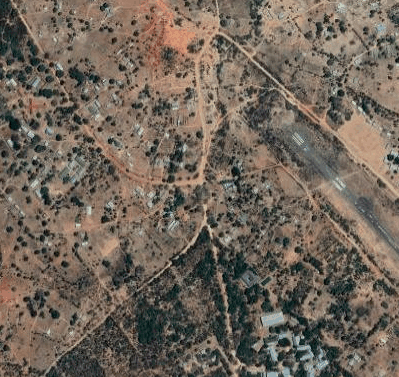
\includegraphics[width=5cm]{low_light.png} }}%
    \qquad
    \subfloat[\centering High light]{{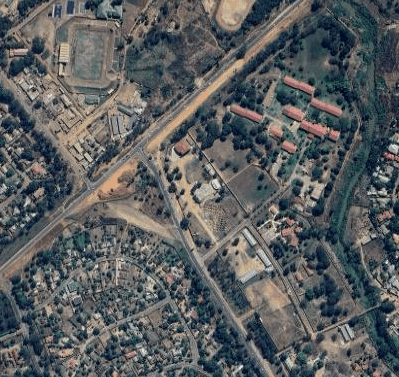
\includegraphics[width=5cm]{high_light.png} }}%
    \caption{Sample from nightlight bins identified by GMM.}%
    \label{fig:example}%
\end{figure}

\subsection{Transfer Learning}

\noindent Now that bins are created and all satellite images are grouped into their respective bins, the first step in model training is to initialize a pre-trained model. In my replication, I deploy the state-of-the-art \textit{VGG11\_BN} developed by \citet{simonyan2014very} using weights that have been pre-trained on the ImageNet database. In the second step, the model is optimized further by training it to predict nightlight intensities from the associated input daytime satellite imagery.

\noindent Here I draw on the Pytorch library which consists of a range of CNN model choices and use the finetuning functions written by \citet{pytut} for implementation. The code was modified so that the first 10 epochs perform fine-tuning - that is, updating all model parameters, and last ten perform feature extraction where only the output layer weights are updated taking the pre-trained model parameters are given. In my configuration, the number of classes is set to 3 since there are 3 nightlight bins and number of epochs set to 2.\footenote{The low number of epochs is a significant limitation on subsequent results, but is necessary due to hardware limitations since even one epoch can take several hours to complete.}

\section{Predicting Poverty using Machine Learning }

\subsection{nightlight Intensity and Consumption}

\noindent We can fit a variety of modern machine learning models to predict consumption expenditures in the data. First, I assess model performance of using nightlight data alone to predict (log) consumption by compare the $R^2$ obtained from Random Forest, LASSO, Ridge, Bayesian Ridge, XGBoost, and a simple linear model. Following the methodology in \citet{jean2016combining}, these models are evaluated using the average $R^2$ across K-fold cross validation. I provide estimates for both 5-fold and 10-fold cross validations.

\begin{table}[H]
\centering
    \scalebox{1.1}{\input{../bld/python/tables/table_ML_estims.tex}}
\caption{Estimates from using ML models to predict consumption from nightlights using $R^2$ as the performance measure.}
\end{table}

\noindent We see from the table that the ridge models are among the best performing along the measure $R^2$.  Moreover, the models tend to do be better on 5-Fold cross validation than 10-Fold. Next we seek to improve these performances by integrating nightlights as an intermediate step in the prediction process instead of using them as a direct predictor of consumption expenditure. 

\subsection{Satellite Imagery and Consumption}

\noindent The trained CNN model is now used to extract feature vectors for each image, which are a nonlinear mapping of the input images to their vector representations. The extraction occurs just before the image classification step. This result is an $n$ x $p$ dimensional matrix, where $n = 11,560$ (all satellite images) and $p = 4096$, the feature vectors for each image. The images were grouped according to their household-clusters and aggregated at this level using the mean. This process reduces the original matrix to $\textbf{X}$, a 780 by 4096 feature matrix, and outcome $\textbf{Y}$ a vector for consumption per capita. The goal is to use these features extracted from satellite images, instead of directly using nightlights, to predict consumption expenditure.

\noindent However, using such a high dimensional dataset for prediction can be problematic and caused convergence issues when training certain ML models such as LASSO. Therefore, instead of using the entire feature matrix for training these models, I first perform dimensionality reduction guided by principal component analysis. The figure below shows the cumulative variance explained by these components. 

\begin{figure}[H]
\centering
    \includegraphics[scale=0.6]{../bld/python/figures/pca.png}
    \caption{Scree plot of first hundred principal components and the cumulative variance.}
    \label{fig:python-predictions}
\end{figure}

\noindent The first hundred components explain 97.5\% of the variation, therefore only these components are retained for model training. ML models are once again used to predict the (log) consumption expenditure.

\begin{table}[H]
\centering
    \scalebox{1.1}{\input{../bld/python/tables/table_CNN_estims.tex}}
	\caption{Estimates from using various ML models to predict consumption per capita using $R^2$ as the performance measure.}
\end{table}

\noindent Overall these ML models trained with features data record higher $R^2$  compared to ML trained with nightlight data, when this measure is computed using 10-Fold cross validation. And perform similarly when computed using 5-Fold cross validation. However, the $R^2$ maxima tend to be higher on ML trained with nightlights data. 

\noindent These results suggest that, in some cases, using information extracted using nightlights data can be more useful than nightlights data itself when quantifying economic outcomes such as consumption expenditure. Therefore, in replicating the study by \citet{jean2016combining}, this project highlights the promising role of satellite imagery for economic analysis. 

\noindent Nonetheless, the project approaches but is not able to replicate the $R^2$ in the original paper. There are various factors that can account for this difference. The first reason is that the results in the original paper for Malawi were based on data from 2013. On the other hand, I use 2016 survey and nightlights data. In addition, the satellite images downloaded were from the most recent years and so it is difficult to quantify how big of a difference this mis-match would have made. Finally, computational bottlenecks limited the number of CNN models I could experiment with and the number of epochs for improving model loss and accuracy. These factors provide avenues for further extensions of the project. 

\setstretch{1}
\printbibliography
\setstretch{1.5}


% \appendix

% The chngctr package is needed for the following lines.
% \counterwithin{table}{section}
% \counterwithin{figure}{section}

\end{document}
